\chapter{Wide Area Network Based Data Center Energy Simulations for Internet Services}
\label{chp:traffic}

\section{Chapter Abstract}
    Data centers are a critical component of modern day economies and social lives of people all around the world. In many aspects society’s dependency on internet services enabled by data centers is still increasing; the COVID-19 stay in place orders are a current example of unprecedented growth rates for many internet services. With the increased dependency on data centers, there is a concern about their environmental impacts across at the globe scale. To reason about the environmental footprint of these globally spanning system requires a new approach to model building energy use of facilities within these systems. This paper demonstrates a top down process that leverages publicly available network traffic data for a globally distributed internet site to model it’s power demand, using Wikipedia as the model internet site. The traffic provides an indication of the building loads that the data center infrastructure must support.  
    
    This chapter demonstrates a method to geographically correlate five data centers with the incoming visits from a global user base using a minimum cost function. The correlations are further extended to provide a forecast of the traffic. The contribution of this research is two-fold. First, it presents a method for a top down assessment of network traffic that can characterize the information technology loads in building energy models. Second, the traffic forecast allows data center operators and designers to model future demands of the building infrastructure systems and perform scenario models based on the projected traffic. 

\section{Introduction}

    Data centers are ubiquitous in today’s society. Consumers of data center enabled web services expect high availability of their functionality and access to their data on a continual basis. These expectations are met with software architectures that provide strongly consistent views of the data regardless of location and in the presence of physical systems failures. In terms of specific failure domains, network failures can be the most catastrophic. For example, an outage of a network link connecting a data center can lead to all physical resources in it to become inaccessible from the outside. With these expectations, the dependencies of internet data centers and their communications network during failures is clearly apparent.
    
    Data center utilities (such as mechanical cooling resources and power distribution resources) and their network connections are not only coupled in failure scenarios described above, but they are also in lock-step with each other through normal operations. This coupling is also easy to reason about; as internet data centers don’t generate workloads hermetically. The workload demands for data centers come from remote consumers (user facing traffic) and other adjacent data centers (back-end traffic). Both forms of incoming traffic instantiate computational and storage processes on the IT hardware, which in turn are powered and cooled by district scale distribution plants.
    
    In the current generation of data centers, the building utility systems demand less than 10\% of the total energy delivered to the site \cite{Shehabi16}. The balance of the power of these new data centers is consumed by the information technology (IT) equipment. With this disproportionate allocation of energy, it is clear that the total energy use in data centers is more sensitive to ITE loads than the facilities systems. Yet the building systems still receive the most attention in the design and facilities operations phase of the buildings. Others have also pointed out similar gaps data center building energy models \cite{Beatty15}. 
    
    To provide an intuition of data center networks, Figure~\ref{net_diag} shows a generalized depiction their topology. At the top are the internet service provider (ISP) networks are shown as clouds because the physical paths of these systems are managed by the global ISPs and they are typically out of control of data center operators. Data center operator’s depend on the ISPs for connecting their facilities through private wide area networks (WAN). The pink lines indicate these wide area connections that traverse over ISP networks. The magenta links connect global WANs data center metropolitan, which typically are responsible for the last miles of network distribution. Within the metropolitan area, their maybe one or more data center sites, only two are shown for clarity in the figure. 
    
    \begin{figure}[h]
\centering
    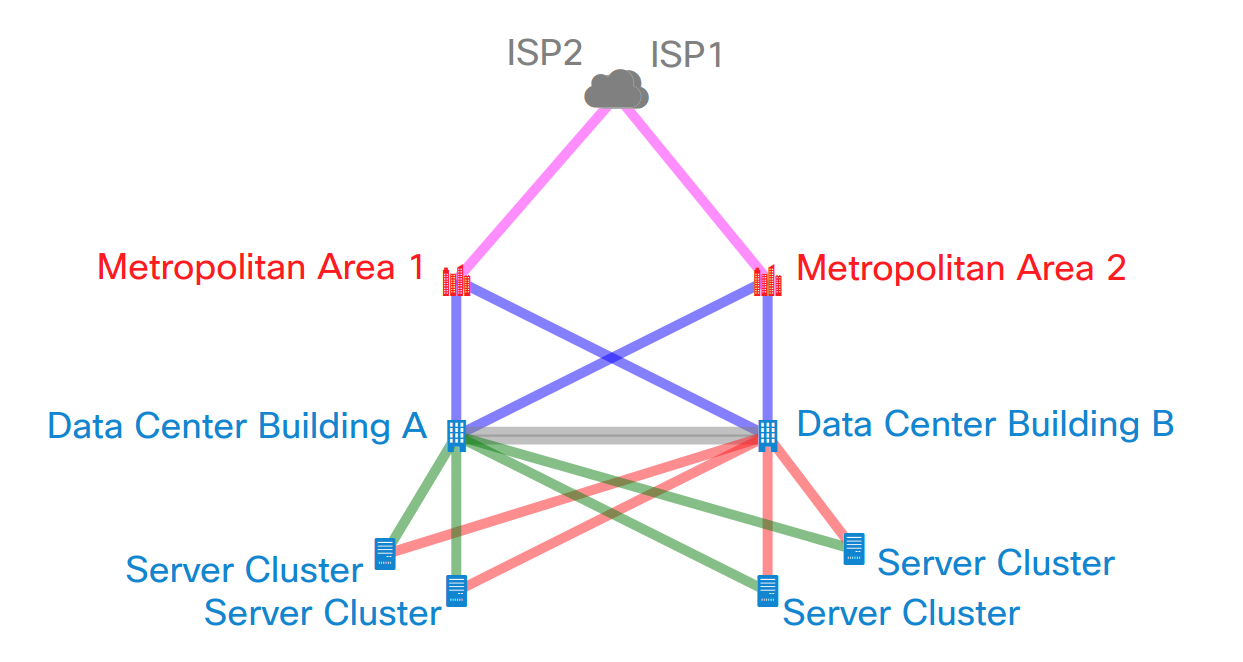
\includegraphics[scale=0.2]{traffic_profile/images/net_diag.png}
    \caption[Network Diagram]{Generic Data Center Network Topology.}
\label{net_diag}
\end{figure}

    
    To motivate business incentives  for  a  more  integrated  IT  and  building model, the  data  center construction spending is estimated to be \$89 billion by 2027, nearly doubling the spend seen in 2018 \cite{dcmarket19}. At the core,the demands for data centers is driven by the expected consumer traffic to its services. With this much value at stake, capital and operational decisions must be based on robust system level models that couple IT traffic and data center designs.
    
\section{Background}
    EnergyPlus, the US Department of Energy’s building energy modeling software has supported data center model since release 8.3. [4]. EnergyPlus modeling engine allows for IT equipment load schedules to be explicitly modeled in it. Today, EnergyPlus comes with three example data center models, in the form of IDF files. These IDFs provide a template that energy analysts can extend and augment to represent their specific data center designs. These default templates are hermetic and lack coordination with the dynamic IT loads. However, there are supplemental software applications that allow external software to integrate with EnergyPlus yielding a robust feedback loop. Building Control Virtual test bed (BCVTB) is one such application \cite{EnergyPlus8.3}. 
    
    \begin{figure}[h]
\centering
    
\includegraphics[scale=0.15]{traffic_profile/images/agent_bem.png}
    \caption[Software Agent and BEM Interaction]{General process flow between EnergyPlus and internet traffic simulation.  .}
\label{agent_bem}
\end{figure}
    
    Wei demonstrates the use of BCVBT in \cite{wei17} for modeling a mixed used facility and has a data center collocated with occupied spaces. Zhang demonstrated the use of BCVBT for control an educational building \cite{zhang19}. Zhang published their Python code base to allow others to replicate their work. Functionally, BCVTB creates an interactive process loop with EnergyPlus allowing the Python program to be aware of EnergyPlus simulations at every simulation time step. Figure 2 illustrates this interactive loop between EnergyPlus and Python. Next, background about wide area network from an internet service perspective is provided. 
    
    Wide area networks serve as the backbone for many internet applications that operate across regionally distributed data centers. The traffic on the inter data center links are segregated into three classes; interactive, large file transfers, and background. Linkedin’s experience with these three classes of traffic is document well by Zhuang \cite{zhuang15}. Interactive traffic consists of blocking operations; where the sequential byte level transactions are required to keep things proceeding. Large file transfers entail transmission of requested resources by some deadline. Background traffic are workloads that opportunistically send traffic and preempting them does not expose the system to any idempotent side effects. Database communications traffic typically consists of workloads that are bound by deadlines and are also pseudo-interactive. These three classes of traffic can either be user facing or back-end. Microsoft and Google have both published their experiences in designing and operating these massive global networks \cite{hong13, sushant13}.  

\section{Methodology} 
    In this section the methods for synthesizing network traffic to correlate it with data center workloads is described. There are four step-wise methods that ultimately yield results that are usable for building energy modeling. These sub-sections first describe the service level data-set that is used throughout this article. Then the service level information is abstracted to indicate network bandwidth, which in turn is correlated with power in the third sub-section. The final method discussed shows a method to scale historical service demands into projection of future loads for data centers.  
    
    \begin{figure}[!htn]
  \subfloat[Mean Value of Page Views]
  {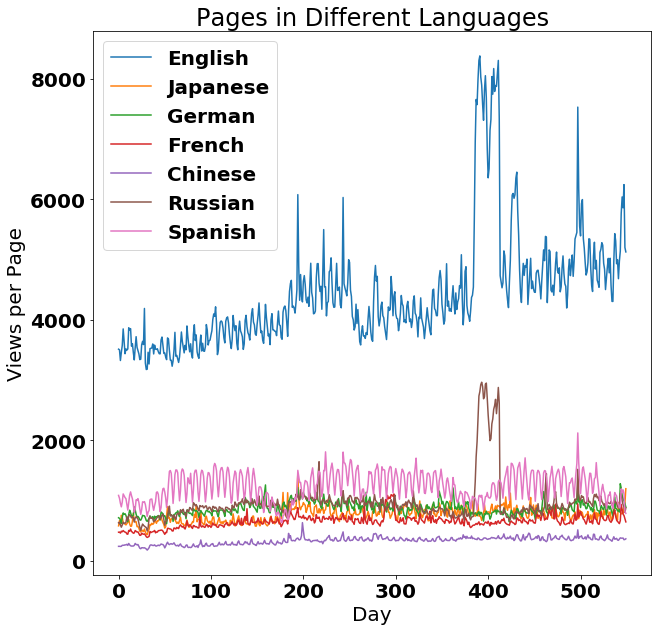
\includegraphics[width=0.5\textwidth]{traffic_profile/images/mean.png}\label{mean}}
  \hfill
  \subfloat[$95^{th}$ Quantile Value of Page Views] 
  {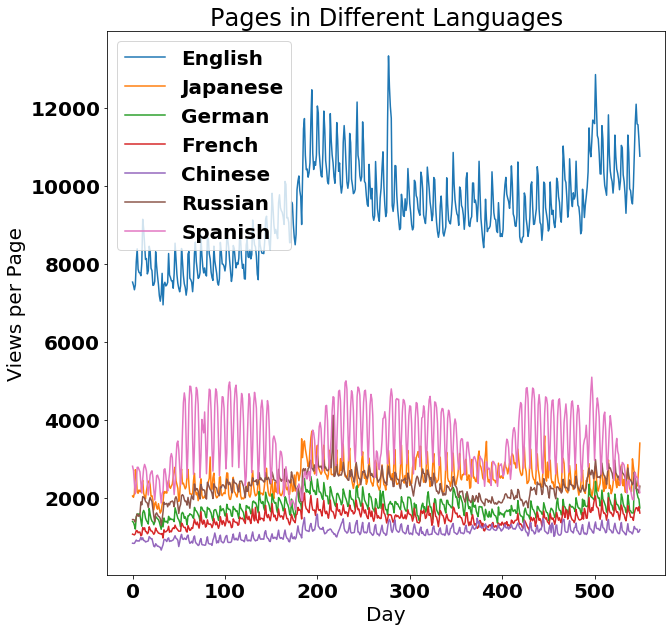
\includegraphics[width=0.5\textwidth]{traffic_profile/images/quantile95_use.png}\label{95thquantile}}
  \caption[Page Views by Language]{Pages Views for Each Language}
\end{figure}

    Traffic to 145,063 Wikipedia Pages for 803 days from July 2015 through September 2017 is used to demonstrate a top-down WAN model for global services. The data is used to train and test the models developed in this section. The training set is partitioned to be inclusive of traffic from July 2015 to December 2016. The remaining data is used to test accuracy of the models. All pages are segregated into 7 different languages; namely English, Japanese, German, French, Chinese, Russian, and Spanish. The mean volume of visits per language is shown in \ref{mean} and the 95th quantile is shown in \ref{95thquantile}.  